\section{Backend}

\subsection{Technologies and libraries}\label{_technologies}

\subsubsection{NodeJs}
Node.js is an open-source, cross-platform, back-end JavaScript runtime environment that runs on the V8 engine and executes JavaScript code outside a web browser. Node.js lets developers use JavaScript to write command line tools and for server-side scripting—running scripts server-side to produce dynamic web page content before the page is sent to the user's web browser. Consequently, Node.js represents a "JavaScript everywhere" paradigm, unifying web-application development around a single programming language, rather than different languages for server-side and client-side scripts.

\begin{itemize}
    \item \textbf{Used Version:} 4.2.2
\end{itemize}

\subsubsection{Typescript}
TypeScript is a programming language developed and maintained by Microsoft. It is a strict syntactical superset of JavaScript and adds optional static typing to the language. TypeScript is designed for the development of large applications and transcompiles to JavaScript.

\begin{itemize}
    \item \textbf{Used Version:} 4.2.2
\end{itemize}

\subsubsection{JSON}
JSON (JavaScript Object Notation) is an open standard file format, and data interchange format, that uses human-readable text to store and transmit data objects consisting of attribute–value pairs and array data types (or any other serializable value). It is a very common data format, with a diverse range of applications, such as serving as a replacement for XML in AJAX systems.


\subsubsection{DynamoDB}
Amazon DynamoDB is a fully managed proprietary NoSQL database service that supports key-value and document data structures and is offered by Amazon.com as part of the Amazon Web Services portfolio.
\subsubsection{Npm}
Npm is the package manager for the Node JavaScript platform. It puts modules in place so that node can find them, and manages dependency conflicts intelligently.
It is extremely configurable to support a wide variety of use cases. Most commonly, it is used to publish, discover, install, and develop node programs.
\subsubsection{Swagger}
Swagger is an Interface Description Language for describing RESTful APIs expressed using JSON. Swagger is used together with a set of open-source software tools to design, build, document, and use RESTful web services. Swagger includes automated documentation, code generation (into many programming languages), and test-case generation.


\subsection{Architecture}\label{_architecture}

\subsubsection{Main components}
We created a serverless and microservices oriented architecture. Each microservice is hosted in a different repository, with its own persistence layer and CI rules.
The microservices created and their respective responsabilities are:
\begin{itemize}
    \item \textbf{products}: you can find the repo \href{https://github.com/SWException/products}{here}; it provides CRUD functionalities for products management,
          like create a new product, modify an existing one, etc... It has also the responsibility to manage images associated to a product, which are
          stored in a Amazon S3 bucket;
    \item \textbf{carts}: you can find the repo \href{https://github.com/SWException/carts}{here}; it has the responsibility to manage carts of all users and guests that
          added some products to their carts. Carts are identified by the user ID (provided by Amazon Cognito), so it communicates with users microservice for each call.
          Each cart contain only an array of tuples composed by a products ID and a quantity (integer);
    \item \textbf{orders}: you can find the repo \href{https://github.com/SWException/orders}{here}; it has the responsibility to provide CRUD functionalities for orders information.
          It also has to provide API's to start and complete checkout process, communicating with Stripe to generate a payment intent;
    \item \textbf{users}: you can find the repo \href{https://github.com/SWException/users}{here}; it provide the functionality to check a Cognito's token JWT to other microservices.
          It also provides to the frontend service the possibility to get the customers list and details about a specific customer;
    \item \textbf{categories}: you can find the repo \href{https://github.com/SWException/categories}{here}; it provides CRUD functionalities to manage categories information.
          This is called, for example, each time that someone asks for product details to the products microservice;
    \item \textbf{taxes}: you can find the repo \href{https://github.com/SWException/taxes}{here}; it provides CRUD functionalities to manage taxes information;
    \item \textbf{addresses}: you can find the repo \href{https://github.com/SWException/addresses}{here}; it provides CRUD functionalities to manage addresses information.
\end{itemize}

\subsubsection{External service}\label{_architectureExternalServices}
In this application, we relied on AWS Cognito service for authentication and Stripe Payment APIs for managing the checkout process.
\paragraph*{AWS Cognito}
Amazon Cognito allows us to implement easily the registratiomn, authentication and user managment.
It can scale resources for milions of users and support thirdy part login (not implemented in our use case).

\paragraph*{Stripe}
Stripe provides APIs that web developers can use to integrate payment processing into their websites and mobile applications.
The advantage of this choice is that our application can be not compliant to security standards required for managing payment card's informations.

\subsection{Class diagrams}\label{_classDiagram}
All services are projected with the same architectural pattern, each one has three layer:
\begin{itemize}
    \item the first contains one handler for each API defined in swagger;
    \item the second is the core and contains model logic;
    \item the third and last is the repository layer, which has the responsibility to interface the
          service with third part services, databases and other services of the backend module.
\end{itemize}
In the following paragraphs, we will present a class diagram for each service.

% ##### CLASS DIAGRAMS #####

\subsubsection{Taxes service}
\begin{figure}[H]
    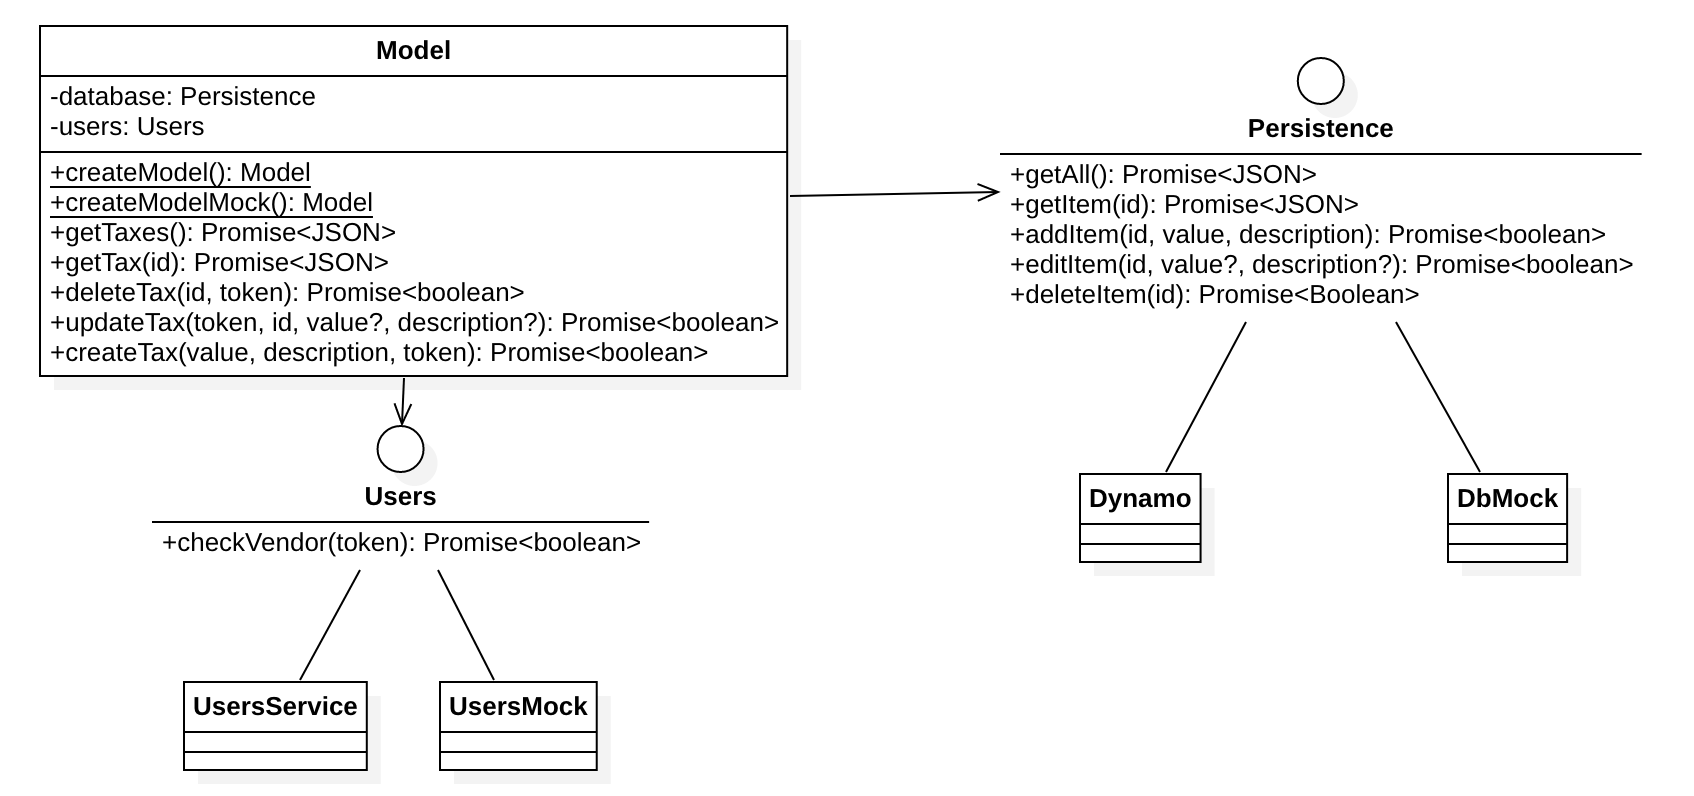
\includegraphics[width=0.9\textwidth]{res/images/class-diagrams/taxes.png}
    \caption{Class UML for taxes service}
\end{figure}
This is the architecture of the service with the responsability to offer CRUD functionalities for taxes management.
The Model class offer to handler functions all the functionalities necessary for their scope. It relies on functionalities
offered by the interfaces Users and Persistence, which have the task to get in touch respectively with the users service and the
database.

\subsubsection{Categories service}
\begin{figure}[H]
    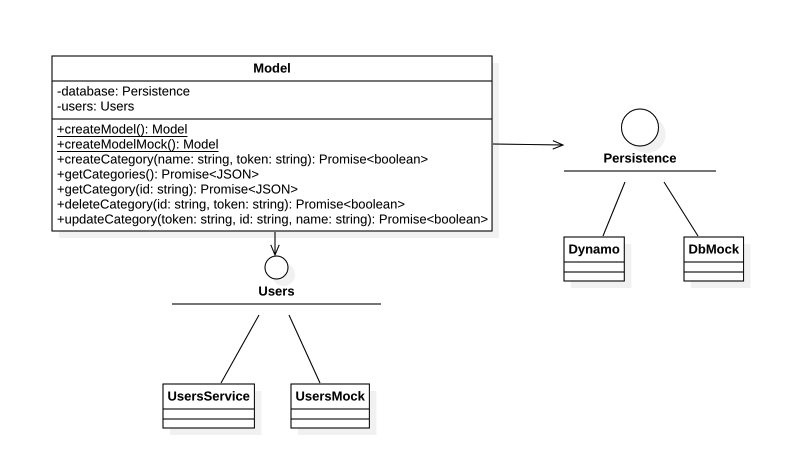
\includegraphics[width=0.9\textwidth]{res/images/class-diagrams/categories.png}
    \caption{Class UML for categories service}
\end{figure}
This diagram shows the classes which exist in Categories service. The architecture is the same as the one in Taxes service,
in fact it offers CRUD functionalities for products' categories.

\subsubsection{Orders service}
\begin{figure}[H]
    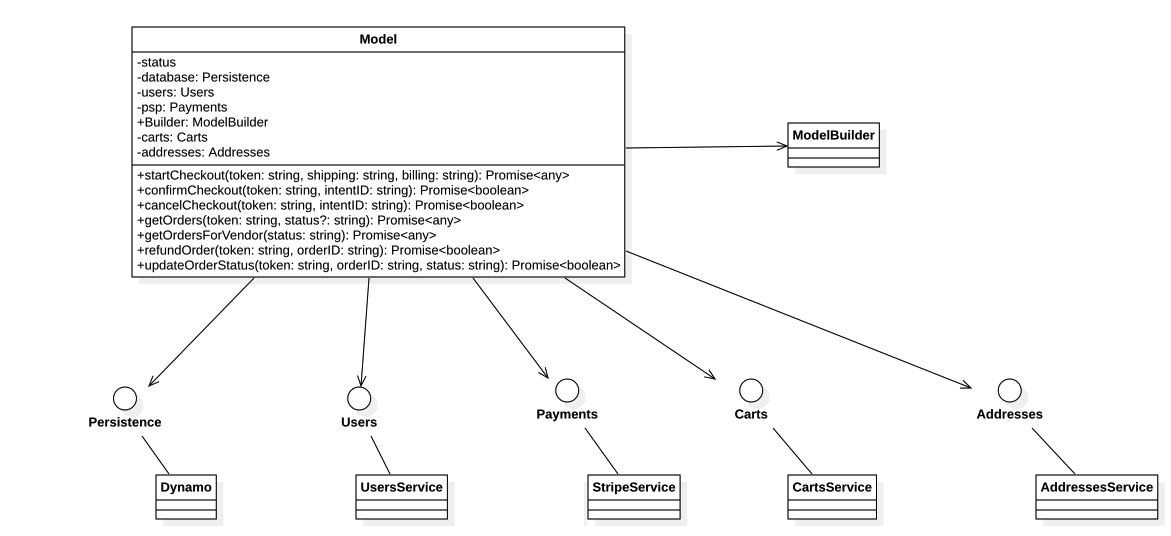
\includegraphics[width=\textwidth]{res/images/class-diagrams/orders.png}
    \caption{Class UML for orders service}
\end{figure}
This service offers CRUD functionalities for orders management. It also exposes API's for managing the checkout process.
The model contains the business logic for implementing all the mentioned functionalities. For these reasons, it relies on a repository layer
which interfaces the service with a persistence layer, the Users service, the Stripe payment service (thirdy part), Carts service and Addresses service.

\subsubsection{Carts service}
\begin{figure}[H]
    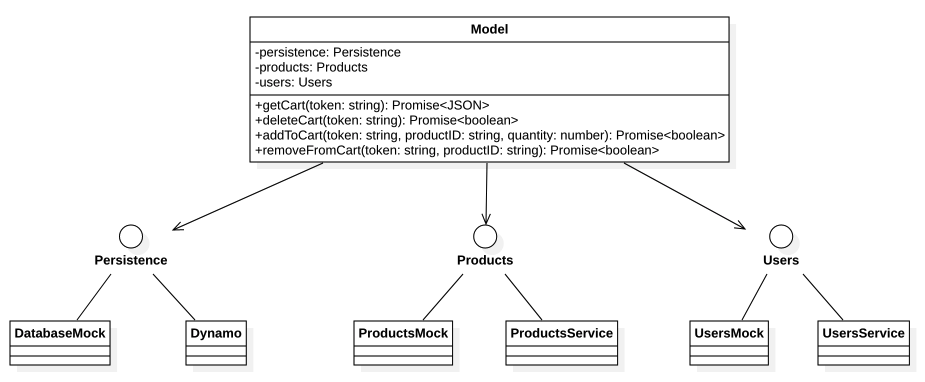
\includegraphics[width=0.9\textwidth]{res/images/class-diagrams/carts.png}
    \caption{Class UML for carts service}
\end{figure}
This service offers CRUD functionalities for carts management, furthermore EML-FE relies on it to add or remove a product in a user's cart.
Since in the cart are saved only the product ID and the relatively quantity, it has to be interfaced with the product service to build an object with complete informations.
This is because a product can be modified by the seller, so the cart must be updated. In this way it get informations just in time.

\subsubsection{Addresses service}
\begin{figure}[H]
    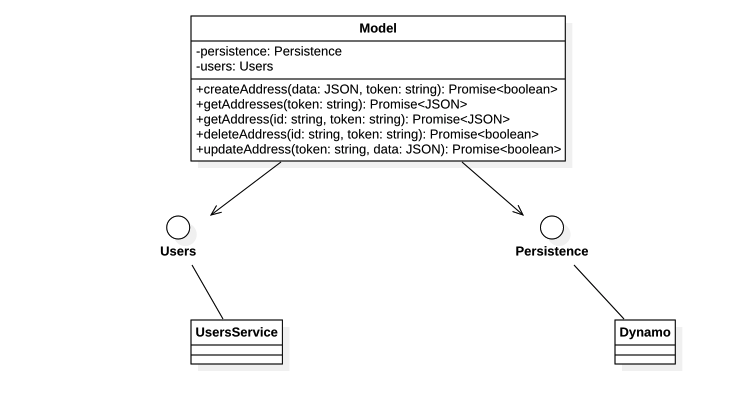
\includegraphics[width=0.9\textwidth]{res/images/class-diagrams/addresses.png}
    \caption{Class UML for addresses service}
\end{figure}
This is the service which has to expose CRUD functionalities for Addresses management. Like other services, it has to be interfaced with Users service to verificate the
autenticity of a token and get the relatively username, so the system can verify that a certain user can access to the requested address. 

\subsubsection{Products service}
\begin{figure}[H]
    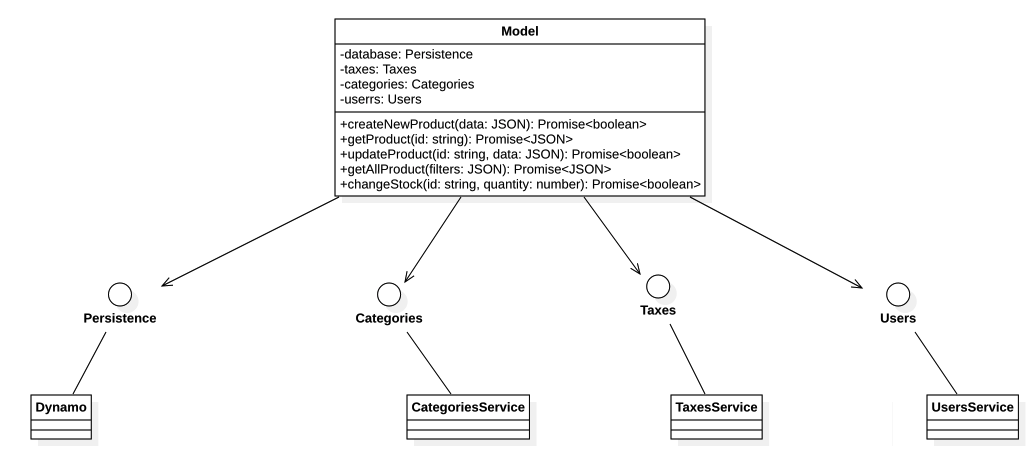
\includegraphics[width=0.9\textwidth]{res/images/class-diagrams/products.png}
    \caption{Class UML for products service}
\end{figure}
The Products service offers CRUD functionalities for managing products informations. It has been interfaced with Categories and Taxes services, so whether a tax value or a category name
is updated it can be updated just in time as well.

\subsubsection{Users service}
\begin{figure}[H]
    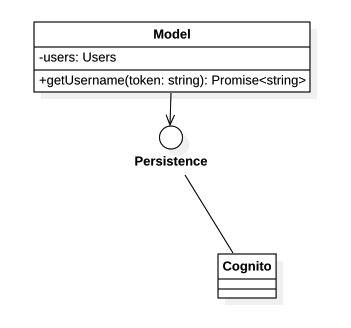
\includegraphics[width=0.45\textwidth]{res/images/class-diagrams/users.png}
    \caption{Class UML for users service}
\end{figure}
The Users service has the responsability to get in touch with AWS Cognito service. Consequently, it is used by all service which have the necessity to verify
a token and/or get a username. It can also provide the information about the user's role.

% #### SEQUENCE DIAGRAMS #######

\subsection{Sequence diagrams} \label{_sequenceDiagram}
In this section we'll provide sequence diagrams for explaining how microservices communicate between one each others when API's are called from the frontend service.

\subsubsection{Taxes service}
\paragraph*{Create tax}
\begin{figure}[H]
    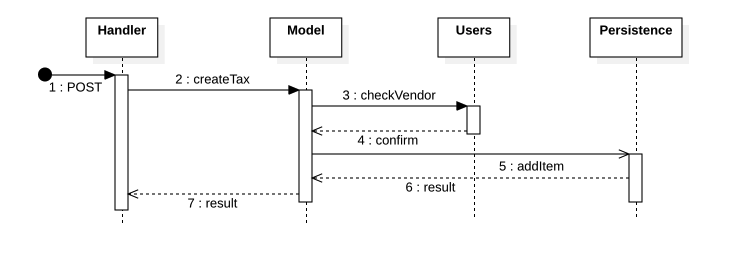
\includegraphics[width=0.9\textwidth]{res/images/sequence-diagrams/taxes/createTax.png}
    \caption{Sequence diagram for createTax API}
\end{figure}
This API is triggered by an HTTP request of type POST with the path /taxes. It is called to create a new tax type in the system. It contacts the Users service through the interface offered by the repository layer to verify
whether a token represent an authenticated vendor.

\paragraph*{Get tax}
\begin{figure}[H]
    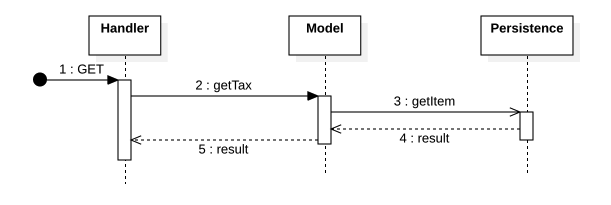
\includegraphics[width=0.9\textwidth]{res/images/sequence-diagrams/taxes/getTax.png}
    \caption{Sequence diagram for getTax API}
\end{figure}
This API is triggered with a GET request to the path /taxes/{id}, where id is a path parameter representing the tax requested. It returns the numeric value of the tax.

\paragraph*{Get taxes}
\begin{figure}[H]
    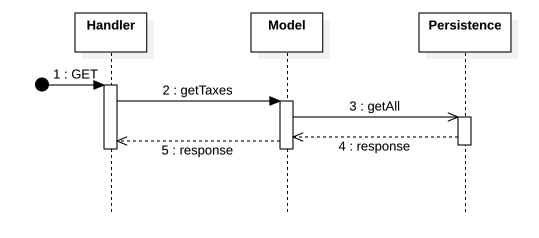
\includegraphics[width=0.8\textwidth]{res/images/sequence-diagrams/taxes/getTaxes.png}
    \caption{Sequence diagram for getTaxes API}
\end{figure}
This API is triggered by a GET request to the path /taxes. It returns all taxes present in the system.

\paragraph*{Update tax}
\begin{figure}[H]
    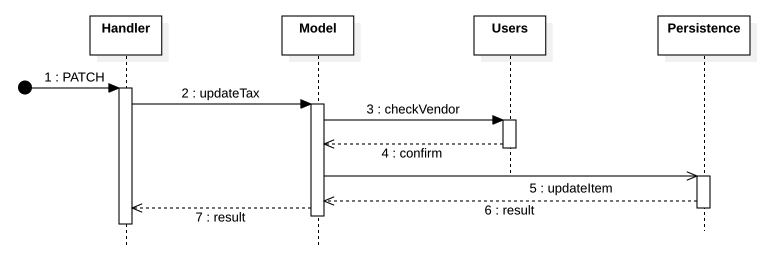
\includegraphics[width=0.8\textwidth]{res/images/sequence-diagrams/taxes/updateTax.png}
    \caption{Sequence diagram for updateTax API}
\end{figure}
This API is called with a PATCH request to the path /taxes/{id}. It is used to update the numeric value of a tax, represented by the id passed in the path parameter.

\paragraph*{Delete tax}
\begin{figure}[H]
    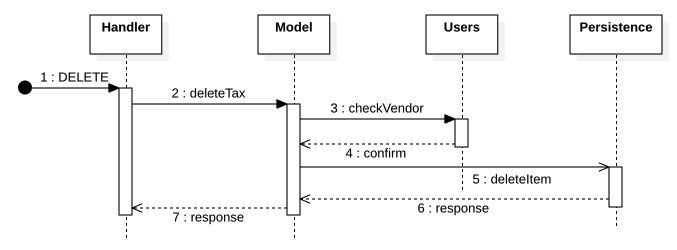
\includegraphics[width=0.9\textwidth]{res/images/sequence-diagrams/taxes/deleteTax.png}
    \caption{Sequence diagram for deleteTax API}
\end{figure}
This API is invocated with a DELETE request to the path /taxes/{id}. It removes from the system the specified tax.

\subsubsection{Categories service}
\paragraph*{Create category}
\begin{figure}[H]
    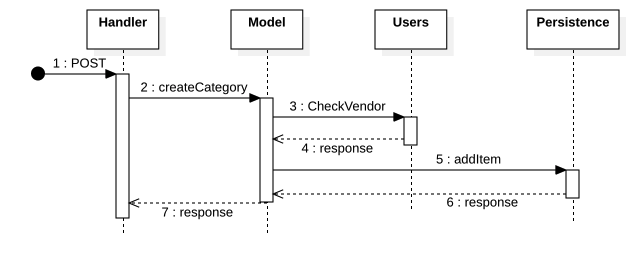
\includegraphics[width=0.9\textwidth]{res/images/sequence-diagrams/categories/createCategory.png}
    \caption{Sequence diagram for createCategory API}
\end{figure}
This API is invocated with a POST request to the path /categories. It create a new category in the system.

\paragraph*{Get categories}
\begin{figure}[H]
    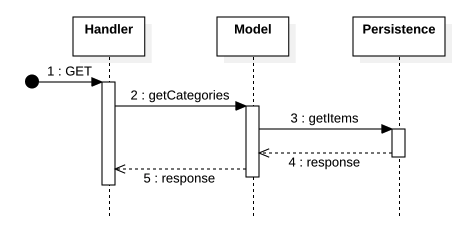
\includegraphics[width=0.8\textwidth]{res/images/sequence-diagrams/categories/getCategories.png}
    \caption{Sequence diagram for getCategories API}
\end{figure}
This API is invocated with a GET request to the path /categories. It returns all categories present in the system.

\paragraph*{Remove category}
\begin{figure}[H]
    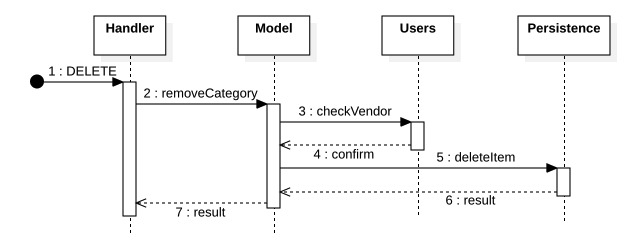
\includegraphics[width=0.9\textwidth]{res/images/sequence-diagrams/categories/removeCategory.png}
    \caption{Sequence diagram for removeCategory API}
\end{figure}
This API is invocated with a DELETE request to the path /categories/{id}. It removes from the system the specified category.

\paragraph*{Update category}
\begin{figure}[H]
    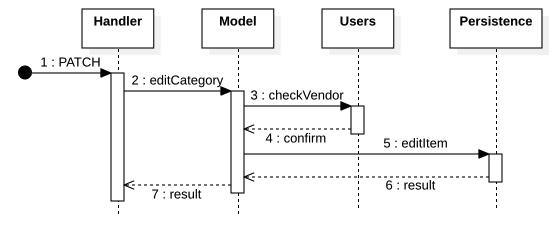
\includegraphics[width=0.9\textwidth]{res/images/sequence-diagrams/categories/updateCategory.png}
    \caption{Sequence diagram for updateCategory API}
\end{figure}
This API is invocated with a PATCH request to the path /categories/{id}. It is used to update the name of the specified category.


\subsubsection{Orders service}
\paragraph*{Get order}
\begin{figure}[H]
    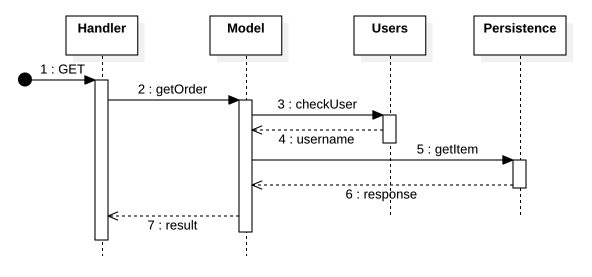
\includegraphics[width=0.9\textwidth]{res/images/sequence-diagrams/orders/getOrderByID.png}
    \caption{Sequence diagram for getOrderByID API}
\end{figure}
This API is invocated with a GET request to the path /orders/{id}. It returns all categories present in the system.

\paragraph*{Start checkout}
\begin{figure}[H]
    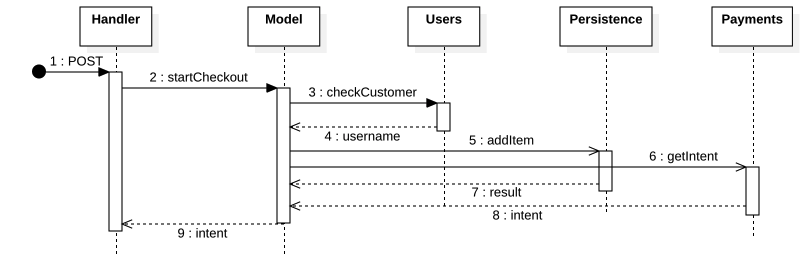
\includegraphics[width=0.9\textwidth]{res/images/sequence-diagrams/orders/startCheckout.png}
    \caption{Sequence diagram for startCheckout API}
\end{figure}
This API is invocated with a POST request to the path /checkout.

\paragraph*{Complete checkout}
\begin{figure}[H]
    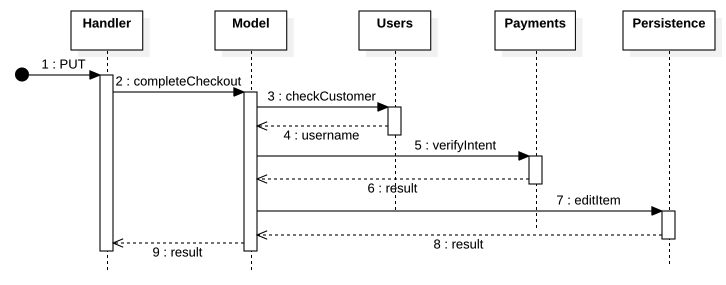
\includegraphics[width=0.9\textwidth]{res/images/sequence-diagrams/orders/completeCheckout.png}
    \caption{Sequence diagram for completeCheckout API}
\end{figure}
This API is invocated with a PUT request to the path /checkout/{intent-id}.

\paragraph*{Cancel checkout}
\begin{figure}[H]
    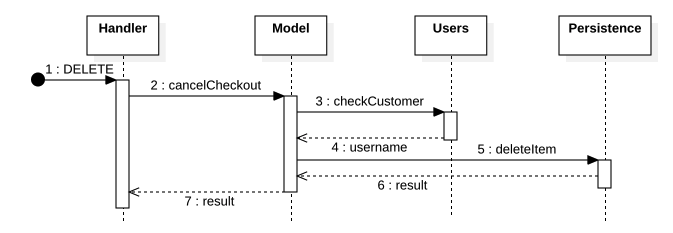
\includegraphics[width=0.9\textwidth]{res/images/sequence-diagrams/orders/cancelCheckout.png}
    \caption{Sequence diagram for cancelCheckout API}
\end{figure}
This API is invocated with a DELETE request to the path /checkout/{intent-id}.

\subsubsection{Carts service}
\paragraph*{Add to cart}
\begin{figure}[H]
    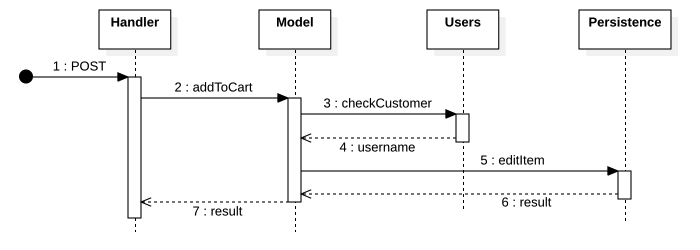
\includegraphics[width=0.9\textwidth]{res/images/sequence-diagrams/carts/addToCart.png}
    \caption{Sequence diagram for addToCart API}
\end{figure}
This API is invocated with a POST request to the path /cart.

\paragraph*{Delete cart}
\begin{figure}[H]
    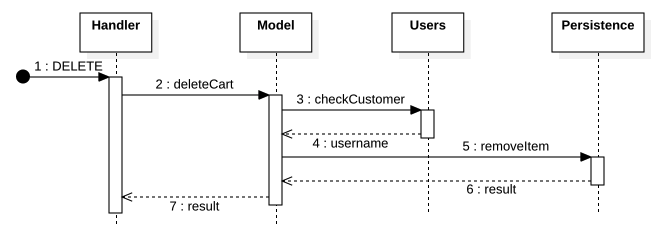
\includegraphics[width=0.9\textwidth]{res/images/sequence-diagrams/carts/deleteCart.png}
    \caption{Sequence diagram for deleteCart API}
\end{figure}
This API is invocated with a DELETE request to the path /cart.

\paragraph*{Get cart}
\begin{figure}[H]
    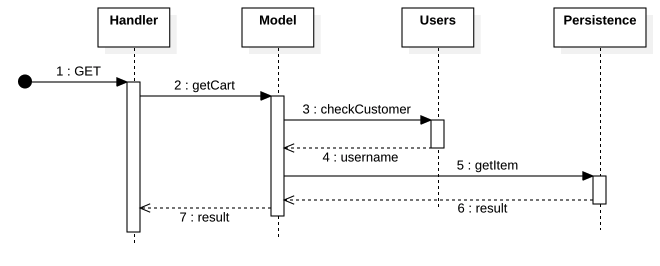
\includegraphics[width=0.9\textwidth]{res/images/sequence-diagrams/carts/getCart.png}
    \caption{Sequence diagram for getCart API}
\end{figure}
This API is invocated with a GET request to the path /cart.

\paragraph*{Remove from cart}
\begin{figure}[H]
    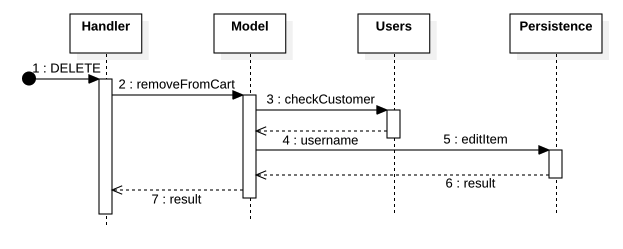
\includegraphics[width=0.9\textwidth]{res/images/sequence-diagrams/carts/removeFromCart.png}
    \caption{Sequence diagram for removeFromCart API}
\end{figure}
This API is invocated with a DELETE request to the path /cart/product/{id}.

\subsubsection{Addresses service}
\paragraph*{Get addresses}
\begin{figure}[H]
    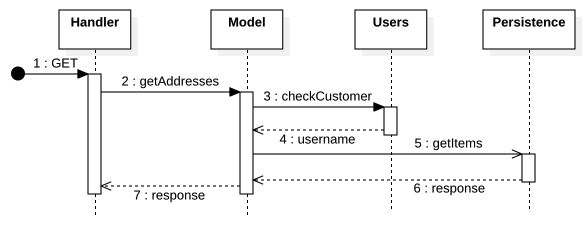
\includegraphics[width=0.9\textwidth]{res/images/sequence-diagrams/addresses/getAddresses.png}
    \caption{Sequence diagram for getAddresses API}
\end{figure}
This API is invocated with a GET request to the path /addresses.

\paragraph*{Insert address}
\begin{figure}[H]
    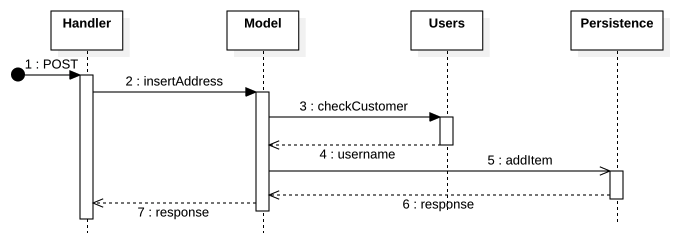
\includegraphics[width=0.9\textwidth]{res/images/sequence-diagrams/addresses/insertAddress.png}
    \caption{Sequence diagram for insertAddress API}
\end{figure}
This API is invocated with a POST request to the path /addresses.

\paragraph*{Remove address}
\begin{figure}[H]
    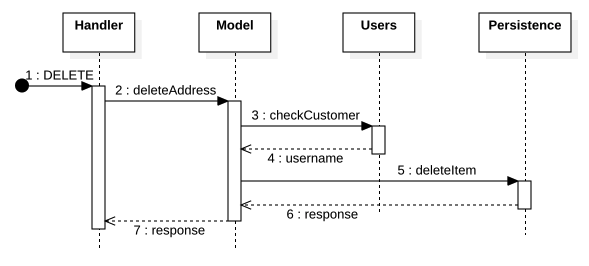
\includegraphics[width=0.9\textwidth]{res/images/sequence-diagrams/addresses/removeAddress.png}
    \caption{Sequence diagram for removeAddress API}
\end{figure}
This API is invocated with a DELETE request to the path /addresses/{id}.

\paragraph*{Update address}
\begin{figure}[H]
    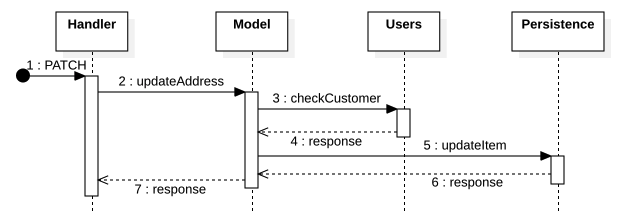
\includegraphics[width=0.9\textwidth]{res/images/sequence-diagrams/addresses/updateAddress.png}
    \caption{Sequence diagram for updateAddress API}
\end{figure}
This API is invocated with a PATCH request to the path /addresses/{id}.


\subsubsection{Products service}
\paragraph*{Get PDP}
\begin{figure}[H]
    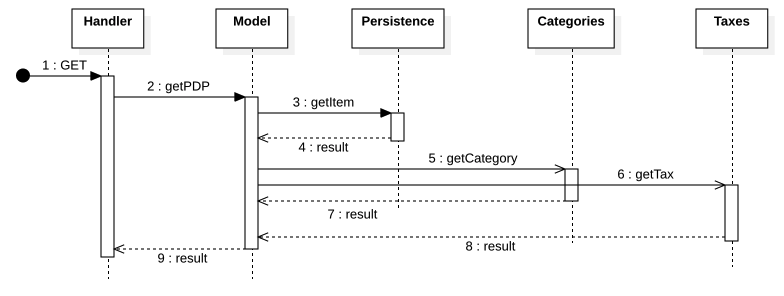
\includegraphics[width=0.9\textwidth]{res/images/sequence-diagrams/products/getPDP.png}
    \caption{Sequence diagram for getPDP API}
\end{figure}
This API is invocated with a GET request to the path /products/{id}.

\paragraph*{Get products}
\begin{figure}[H]
    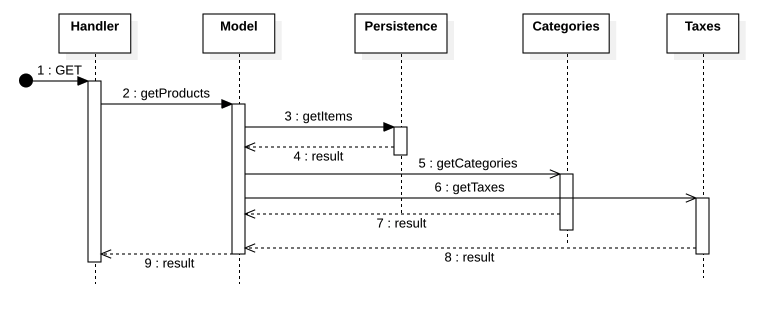
\includegraphics[width=0.9\textwidth]{res/images/sequence-diagrams/products/getProducts.png}
    \caption{Sequence diagram for getProducts API}
\end{figure}
This API is invocated with a GET request to the path /products.

\paragraph*{Edit product}
\begin{figure}[H]
    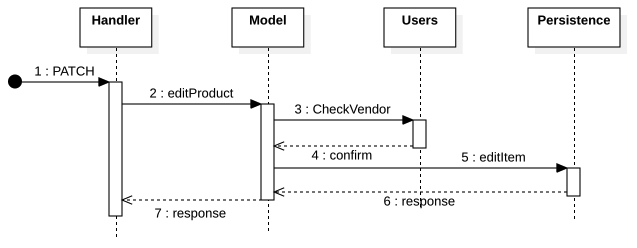
\includegraphics[width=0.9\textwidth]{res/images/sequence-diagrams/products/editProduct.png}
    \caption{Sequence diagram for editProduct API}
\end{figure}
This API is invocated with a PATCH request to the path /products/{id}.

\paragraph*{Create product}
\begin{figure}[H]
    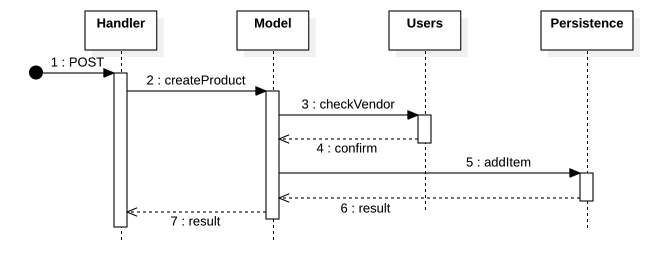
\includegraphics[width=0.9\textwidth]{res/images/sequence-diagrams/products/createProduct.png}
    \caption{Sequence diagram for createProduct API}
\end{figure}
This API is invocated with a POST request to the path /products.

\paragraph*{Remove product}
\begin{figure}[H]
    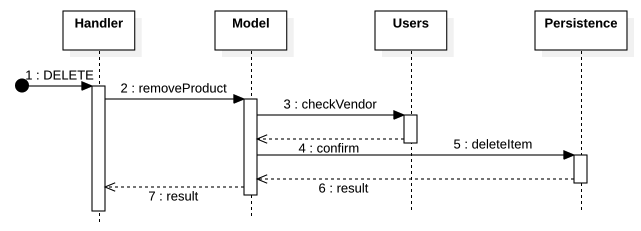
\includegraphics[width=0.9\textwidth]{res/images/sequence-diagrams/products/removeProduct.png}
    \caption{Sequence diagram for removeProduct API}
\end{figure}
This API is invocated with a DELETE request to the path /products/{id}.


\subsubsection{Users service}
\paragraph*{Check customer}
\begin{figure}[H]
    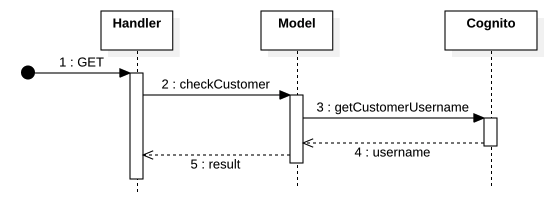
\includegraphics[width=0.9\textwidth]{res/images/sequence-diagrams/users/checkCustomer.png}
    \caption{Sequence diagram for checkCustomer API}
\end{figure}
This API is invocated with a GET request to the path /users/customers/check/{token}.
